\documentclass[journal]{IEEEtran}

% --- Packages ---
\usepackage[T1]{fontenc}
\usepackage[utf8]{inputenc}
\usepackage{cite}
\usepackage{amsmath,amssymb,amsfonts}
\usepackage{graphicx}
\usepackage{xcolor}
\usepackage{hyperref}
\usepackage{booktabs}
\usepackage{multirow}
\usepackage{tabularx}
\usepackage{listings}
\usepackage{microtype}
\usepackage{siunitx}
\usepackage{url}

% --- Hyperref config ---
\hypersetup{
  colorlinks = true,
  linkcolor  = blue,
  citecolor  = blue,
  urlcolor   = blue,
}

% --- Listings config ---
\lstset{
  basicstyle   = \ttfamily\scriptsize,
  breaklines   = true,
  captionpos   = b,
  frame        = single,
  numbers      = none,
  tabsize      = 2,
  showstringspaces = false,
}

% --- Custom commands ---
\newcommand{\todo}[1]{\textcolor{red}{[TODO: #1]}}
\newcommand{\xheep}{X-HEEP}

% =========================================================
\begin{document}

\title{Hardware Processing Engines on FPGA:\\
       A Survey of Open-Source RISC-V Platforms}

\author{
  \IEEEauthorblockN{Krutarth Patel}
  \IEEEauthorblockA{%
    EE23B137, IIT Madras\\
    Supervisors: Dr.\ G.\ Srinivasan, Dr.\ K.\ Sankaranarayanan, Prof.\ N.\ Chandrachoodan\\
    ee23b137@smail.iitm.ac.in}
}

\maketitle

% =========================================================
\begin{abstract}
Custom, low-cost hardware for AI inference is a major research challenge
driven by growing industry demand for edge deployment. Numerous open-source
platforms exist for this purpose. This report documents a three-month survey (February--May 2026)
of candidate platforms for running a Hardware Processing Engine (HWPE) on an
FPGA, conducted as part of the UGRC project at IIT Madras. We evaluated the
Google Coral NPU, the PULP Platform (PULPissimo), and several PULP-derived
alternatives, documenting the specific technical barriers that prevented
deployment in each case. We conclude with a working system built around
X-HEEP extended with the Quadrilatero systolic-array co-processor, which
achieves simulation-verified matrix multiply and convolution workloads. We
identify and fix an RTL handshake deadlock in Quadrilatero that prevented
any result from being produced, and provide a fully reproducible Docker-based
build environment.
\end{abstract}

\begin{IEEEkeywords}
RISC-V, hardware accelerator, systolic array, FPGA, HWPE, CV-X-IF,
X-HEEP, Quadrilatero, edge AI.
\end{IEEEkeywords}

% =========================================================
\section{Introduction}
\label{sec:intro}
The past decade has seen widespread adoption of machine learning across almost every domain.
A recurring challenge in deploying these models is satisfying the power and area constraints imposed
by the target environment. Embedded and edge devices in particular demand compute units that are both
efficient and small. Numerous hardware platforms and software toolchains have been developed to address this,
but the landscape is fragmented and difficult to navigate.

From the perspective of a researcher trying to build and deploy an application, the number of options is
overwhelming. The central question this study addresses is:

\emph{Can a modern, open-source RISC-V SoC be
extended with a hardware accelerator, programmed using a software toolchain,
and demonstrated on an FPGA?}

We constrain ourselves to open-source software and hardware to avoid a dependency on institutional
licences or proprietary tools. We further require that the hardware platform support widely-available
educational FPGAs. These are arguably the minimum requirements for reproducible research.

We evaluate four candidate platforms: Google Coral NPU,
PULPissimo, a cohort of PULP-derived alternatives, and X-HEEP with
the Quadrilatero systolic-array co-processor. For each platform we document the
specific issues encountered and whether they were resolved. Sections~\ref{sec:coral}
through~\ref{sec:alternatives} cover the rejected platforms.
Section~\ref{sec:xheep} covers X-HEEP+Quadrilatero in detail.
Section~\ref{sec:bug} documents the RTL bug found and fixed in Quadrilatero.
Section~\ref{sec:results} presents the experimental results, and
Section~\ref{sec:conclusion} concludes.

% =========================================================
\section{Platform Selection Criteria}
\label{sec:criteria}

Table~\ref{tab:designspace} lists the major axes of the design space across the platforms
surveyed for this project. The list is not exhaustive.

\begin{table}[htbp]
  \centering
  \caption{edge-AI hardware design space.}
  \label{tab:designspace}
  \begin{tabular}{@{}ll@{}}
    \toprule
    \textbf{Axis} & \textbf{Representative options} \\
    \midrule
    CPU core      & CV32E40PX, Snitch, CVA6, Ibex \\
    Accelerator   & Quadrilatero, Gemmini, ITA, RedMulE \\
    Interface     & CV-X-IF, HWPE-Stream, AXI \\
    FPGA target   & Nexys-A7, Genesys2, ZCU102, PYNQ-Z2 \\
    Compiler      & GCC, LLVM/Clang, TVM, Deeploy \\
    Simulator     & Verilator, QuestaSim, GVSoC \\
    \bottomrule
  \end{tabular}
\end{table}

Given the constraints described in Section~\ref{sec:intro}, three
criteria were chosen for evaluating a given platform:

\begin{enumerate}
  \item \textbf{FPGA support.} The platform must be synthesisable on the
        Nexys-A7-100t or Nexys-A7-200t without proprietary EDA licences.
  \item \textbf{Open-source toolchain.} Compilation, simulation, and
        programming must be achievable with freely available tools.
  \item \textbf{Accelerator integration.} The SoC must provide a
        well-documented mechanism for attaching a custom HWPE.
\end{enumerate}

% =========================================================
\section{Platform 1: Google Coral NPU}
\label{sec:coral}

\subsection{Background}

Google Coral is an edge-AI hardware ecosystem centred on a purpose-built
Neural Processing Unit (NPU). It exposes a Python API for running
TensorFlow Lite models and is designed for rapid prototyping of neural
network inference on embedded hardware.

\subsection{Evaluation and Issues}

Coral was evaluated in February 2026 as a potential baseline. The evaluation
was brief: none of the three selection criteria could be satisfied.

\begin{itemize}
  \item \textbf{No FPGA flow.} Coral is a proprietary ASIC. There is no
        RTL netlist and no synthesis flow. The NPU cannot be replicated or
        studied on an FPGA.
  \item \textbf{Closed architecture.} The NPU's microarchitecture is not
        documented. Extending it or understanding its performance
        characteristics requires reverse engineering.
  \item \textbf{No custom-ISA support.} Workloads must reach the NPU
        through the TFLite-to-Coral compiler. There is no mechanism for
        adding custom instructions or attaching a custom accelerator.
\end{itemize}

\subsection{Verdict}

Against the three criteria from Section~\ref{sec:criteria}:

\begin{enumerate}
  \item \textbf{FPGA support.} Not satisfied. Coral is a proprietary ASIC
        with no RTL or synthesis flow.
  \item \textbf{Open-source toolchain.} Partially satisfied for standard
        models via TFLite, but the NPU internals are closed and
        undocumented.
  \item \textbf{Accelerator integration.} Not satisfied. The platform
        does not support custom instructions or external accelerators.
\end{enumerate}

Coral was abandoned. It fails all three criteria and there is no path to making it
work within the constraints of this project.

% =========================================================
\section{Platform 2: PULPissimo}
\label{sec:pulpissimo}

\subsection{Background}

PULPissimo is a microcontroller SoC from ETH Zurich's PULP (Parallel Ultra
Low Power) Platform~\cite{schiavone2017slow}. It features a RISC-V core
and is designed to interface with HWPEs through the standardised HWPE-Stream
interface~\cite{conti2018xne}. It has been widely used in embedded AI
research and is the most established open-source platform for HWPE work.
The platform nominally supports several FPGA boards including the Genesys2
and Nexys families.

\subsection{Evaluation and Issues}

Setup was attempted on a modern Ubuntu~22.04 host in early March 2026. When
that failed, progressively older environments were tried: Ubuntu~20.04 via
a community Docker image (\texttt{patata0717/pulpissimo}). Within the
Docker container, the PULP SDK compiled and RISC-V code could be emulated
using GVSoC, the PULP virtual-platform emulator. RTL simulation could not
be achieved.

\subsubsection{SDK End-of-Life}

The main branch of PULPissimo carries no active software SDK. The
\texttt{pulp-sdk} requires \texttt{gcc-5}, which is packaged only for
Ubuntu~18. Attempting to build on Ubuntu~20 or~22 fails with
incompatible toolchain errors. The last tagged release (June 2021) reduces
but does not eliminate dependency conflicts.

\subsubsection{RTL Simulation Requires QuestaSim}

The \texttt{common\_cells} library used throughout PULPissimo's RTL employs
SystemVerilog testbench features (randomisation, coverage, assertions):

\begin{lstlisting}
** Error: ../ips/common_cells/src/id_queue.sv(278):
Questa has encountered an unexpected internal error.
\end{lstlisting}

ModelSim's trial version does not support these features; QuestaSim (the
commercial edition, requiring a licence) is required. Verilator is not
officially supported by PULPissimo.

\subsection{Verdict}

Against the three criteria from Section~\ref{sec:criteria}:

\begin{enumerate}
  \item \textbf{FPGA support.} Nominally present in older documentation, but
        the supported boards (Genesys2, ZCU102) were not available in the lab,
        and the synthesis flow was never verified with the current codebase.
  \item \textbf{Open-source toolchain.} Not satisfied. RTL simulation requires
        QuestaSim, a commercial tool requiring a paid licence. Verilator is not
        officially supported. The software SDK requires \texttt{gcc-5} on
        Ubuntu~18, making it unusable.
  \item \textbf{Accelerator integration.} Possible in principle via HWPE-Stream,
        but unreachable in practice without a working simulation environment.
\end{enumerate}

PULPissimo was abandoned. The hardware design is sound, but failing criteria
(2) alone is sufficient to make the platform impractical for reproducible
research.

% =========================================================
\section{Platform 3: PULP-Derived Alternatives}
\label{sec:alternatives}

Following the decision to target platforms compatible with the Deeploy
compiler framework~\cite{deeploy2024}, a broader survey of PULP-derived
alternatives was conducted in late March 2026.
Table~\ref{tab:alternatives} summarises the findings.

\begin{table}[htbp]
  \centering
  \caption{PULP-derived platform survey. FPGA col.: first-class support;
           Sim col.: Verilator or equivalent open simulator.}
  \label{tab:alternatives}
  \begin{tabular}{@{}lccp{3.2cm}@{}}
    \toprule
    \textbf{Platform} & \textbf{FPGA} & \textbf{Sim} & \textbf{Blocker} \\
    \midrule
    Chimera       & --  & --  & No FPGA flow; docs insufficient. \\
    Siracusa      & --  & --  & No public repository. \\
    Mempool + ITA & --  & \checkmark & 256 cores; FPGA infeasible. \\
    Snitch Cluster& --  & \checkmark & No out-of-the-box FPGA flow. \\
    GAP9          & N/A & N/A & Proprietary; not open-source. \\
    Cheshire      & \checkmark & \checkmark & No Deeploy backend. \\
    \bottomrule
  \end{tabular}
\end{table}

\subsubsection{Chimera}

Chimera is a template architecture for multi-HWPE pipelines and has been
used in transformer-accelerator research. However, it lacks documentation
for the parts relevant to this project, and no FPGA synthesis flow exists.

\subsubsection{Mempool and ITA}

Mempool is a 256-core RISC-V mesh processor. At full scale, FPGA synthesis
is infeasible. A scaled-down variant (\texttt{minpool}, 16 cores) supports
Verilator but has no FPGA flow.

\subsubsection{Snitch Cluster}

Snitch provides a clean Docker image and Verilator support but is designed
primarily for simulation-first and ASIC workflows. Porting to the available
FPGA boards would require substantial effort.

\subsubsection{Cheshire}

Cheshire is a Linux-capable RISC-V SoC with FPGA support on several boards
and serves as the substrate on which Chimera is built. It came closest to
satisfying the criteria but lacks a Deeploy compiler backend, which would be
required for the software-stack goal of the project.

\subsection{Summary}

Every platform surveyed here lacked either a ready-made FPGA synthesis flow,
a working accelerator integration path, or both. X-HEEP, found at the end of March 2026,
addresses both gaps.

% =========================================================
\section{Platform 4: X-HEEP + Quadrilatero}
\label{sec:xheep}

\subsection{System Overview}

\textbf{X-HEEP} (eXtensible Heterogeneous Energy-Efficient Platform) is a
configurable RISC-V microcontroller developed at EPFL's ESL
lab~\cite{xheep2023}. It is built around the CV32E40PX core (a 32-bit,
four-stage in-order processor) and is purpose-designed for extensibility:
a co-processor can be attached through the \textbf{CV-X-IF}
interface~\cite{cvxif_spec} without modifying any MCU RTL. X-HEEP ships
with first-class FPGA support for the Nexys-A7, Genesys2, ZCU102, and
PYNQ-Z2 boards, and an active Docker-based build system.

\textbf{Quadrilatero}~\cite{quadrilatero2021} is a systolic-array
co-processor implementing the custom \texttt{xtheadmatrix} RISC-V ISA
extension for matrix operations. The 4$\times$4 systolic array is a
weight-static design inspired by the Register-Aware Systolic Array (RASA)
architecture~\cite{rasa2021}. It connects to X-HEEP through CV-X-IF,
enabling the CPU to dispatch matrix instructions directly to the
accelerator. Quadrilatero includes its own Load-Store Unit (LSU) with
direct memory access, making it semi-autonomous once an instruction is
accepted.

\subsection{What X-HEEP Does Right}

\subsubsection{FPGA-First Design}

Unlike the platforms surveyed earlier, X-HEEP treats FPGA deployment as a
primary target rather than an afterthought. Synthesis scripts are maintained
for multiple boards and updated with each release. The bitstream generation
command is a single \texttt{make} invocation:

\begin{lstlisting}
make vivado-fpga FPGA_BOARD=nexys-a7-200t
\end{lstlisting}

\subsubsection{CV-X-IF: A Clean Accelerator Interface}

The CV-X-IF interface~\cite{cvxif_spec} decouples the CPU pipeline from the
co-processor completely. The CPU offloads custom instructions without stalling
the pipeline (assuming the co-processor responds promptly with an
\texttt{accept} signal), and the co-processor writes results back through a
separate result channel. This means Quadrilatero can be integrated into
X-HEEP without touching any MCU RTL, which is a significant advantage over
tightly-coupled HWPE-Stream designs where the accelerator must be wired into
the SoC fabric directly.

\subsubsection{Active Docker Toolchain}

X-HEEP provides an official \texttt{x-heep-toolchain} Docker image that
packages Verilator, FuseSoC, and all MCU dependencies. In contrast to
PULPissimo, the simulation flow uses Verilator, which is freely available
and actively maintained. The image is regularly updated and tested against
the current X-HEEP codebase.

\subsection{Environment Setup}
\label{subsec:env}

A custom \texttt{Dockerfile} was written on top of \texttt{x-heep-toolchain}
to add the libraries required to run Vivado inside the container. Vivado
itself is \emph{mounted} as an external volume at runtime rather than bundled
into the image, keeping the image size manageable and allowing different
Vivado versions to be used without rebuilding.

\paragraph{Vivado Version Issue}

The X-HEEP FPGA TCL scripts use the \texttt{-freq\_hz} flag in
\texttt{create\_bd\_port}, which was introduced after Vivado~2018.3. The
initially available installation was version~2018.3:

\begin{lstlisting}
Unknown option '-freq_hz', please type
'create_bd_port -help' for usage info.
while executing "source xilinx_generate_clk_wizard.tcl"
\end{lstlisting}

\paragraph{Resolution} A Vivado~2022.1 installation was mounted into the
container. Once the correct version was in place, MCU generation and
bitstream synthesis completed successfully.

\subsection{Verilator Simulation}
\label{subsec:verilator}

The X-HEEP simulation model is compiled using FuseSoC and Verilator. The
first attempt to compile the model for the X-HEEP+Quadrilatero configuration
failed with:

\begin{lstlisting}
%Error: Exiting due to 1 warning(s) [COMBDLY]
\end{lstlisting}

Verilator~5.x promotes a non-blocking assignment inside a combinational
block to an error by default. The offending line is in the CV32E40PX
behavioural clock-gate model:

\begin{lstlisting}
if (clk_i == 1'b0) clk_en <= en_i | scan_cg_en_i;
\end{lstlisting}

\paragraph{Resolution} A \texttt{/* verilator lint\_off COMBDLY */} guard
was applied around the offending line in the vendored copy of the behavioural
model. The simulation then compiled and ran cleanly.

\subsection{Custom LLVM Compiler Toolchain}
\label{subsec:toolchain}

The \texttt{xtheadmatrix} ISA extension used by Quadrilatero is not present
in upstream LLVM or GCC. A patched LLVM must be built from the
\texttt{xheep\_matrix\_spec} repository~\cite{xheep_matrix_spec}. The build
process first compiles \texttt{riscv-gnu-toolchain} and
then builds LLVM with the custom RISC-V backend. The toolchain is installed
into a user-owned host directory that is mounted into the container, so it
persists across container runs.

Applications targeting Quadrilatero are compiled with:

\begin{lstlisting}
make app PROJECT=example_matmul_quadrilatero \
  ARCH=rv32imc_zicsr_xtheadmatrix0p1 \
  COMPILER_FLAGS=-menable-experimental-extensions \
  COMPILER=clang CLANG_LINKER_USE_LD=1
\end{lstlisting}

\subsection{Verification}
\label{subsec:ifverify}

A matrix multiplication application was compiled and simulated under
Verilator. GTKWave was used to inspect the waveforms. The CV-X-IF
transaction sequence was verified:

\begin{enumerate}
  \item The CPU correctly dispatches every \texttt{xtheadmatrix} instruction
        over CV-X-IF. The offload request channel shows valid opcodes and the expected register addresses.
  \item Quadrilatero accepts each instruction (\texttt{accept~=~1} on the
        issue channel).
  \item \textbf{The result-valid signal is never asserted.}
\end{enumerate}

The third observation is not an interface error but an internal failure,
and is the subject of Section~\ref{sec:bug}.

% =========================================================
\section{The Quadrilatero Handshake Bug}
\label{sec:bug}

\subsection{Default Behaviour}

\begin{figure*}[t]
  \centering
  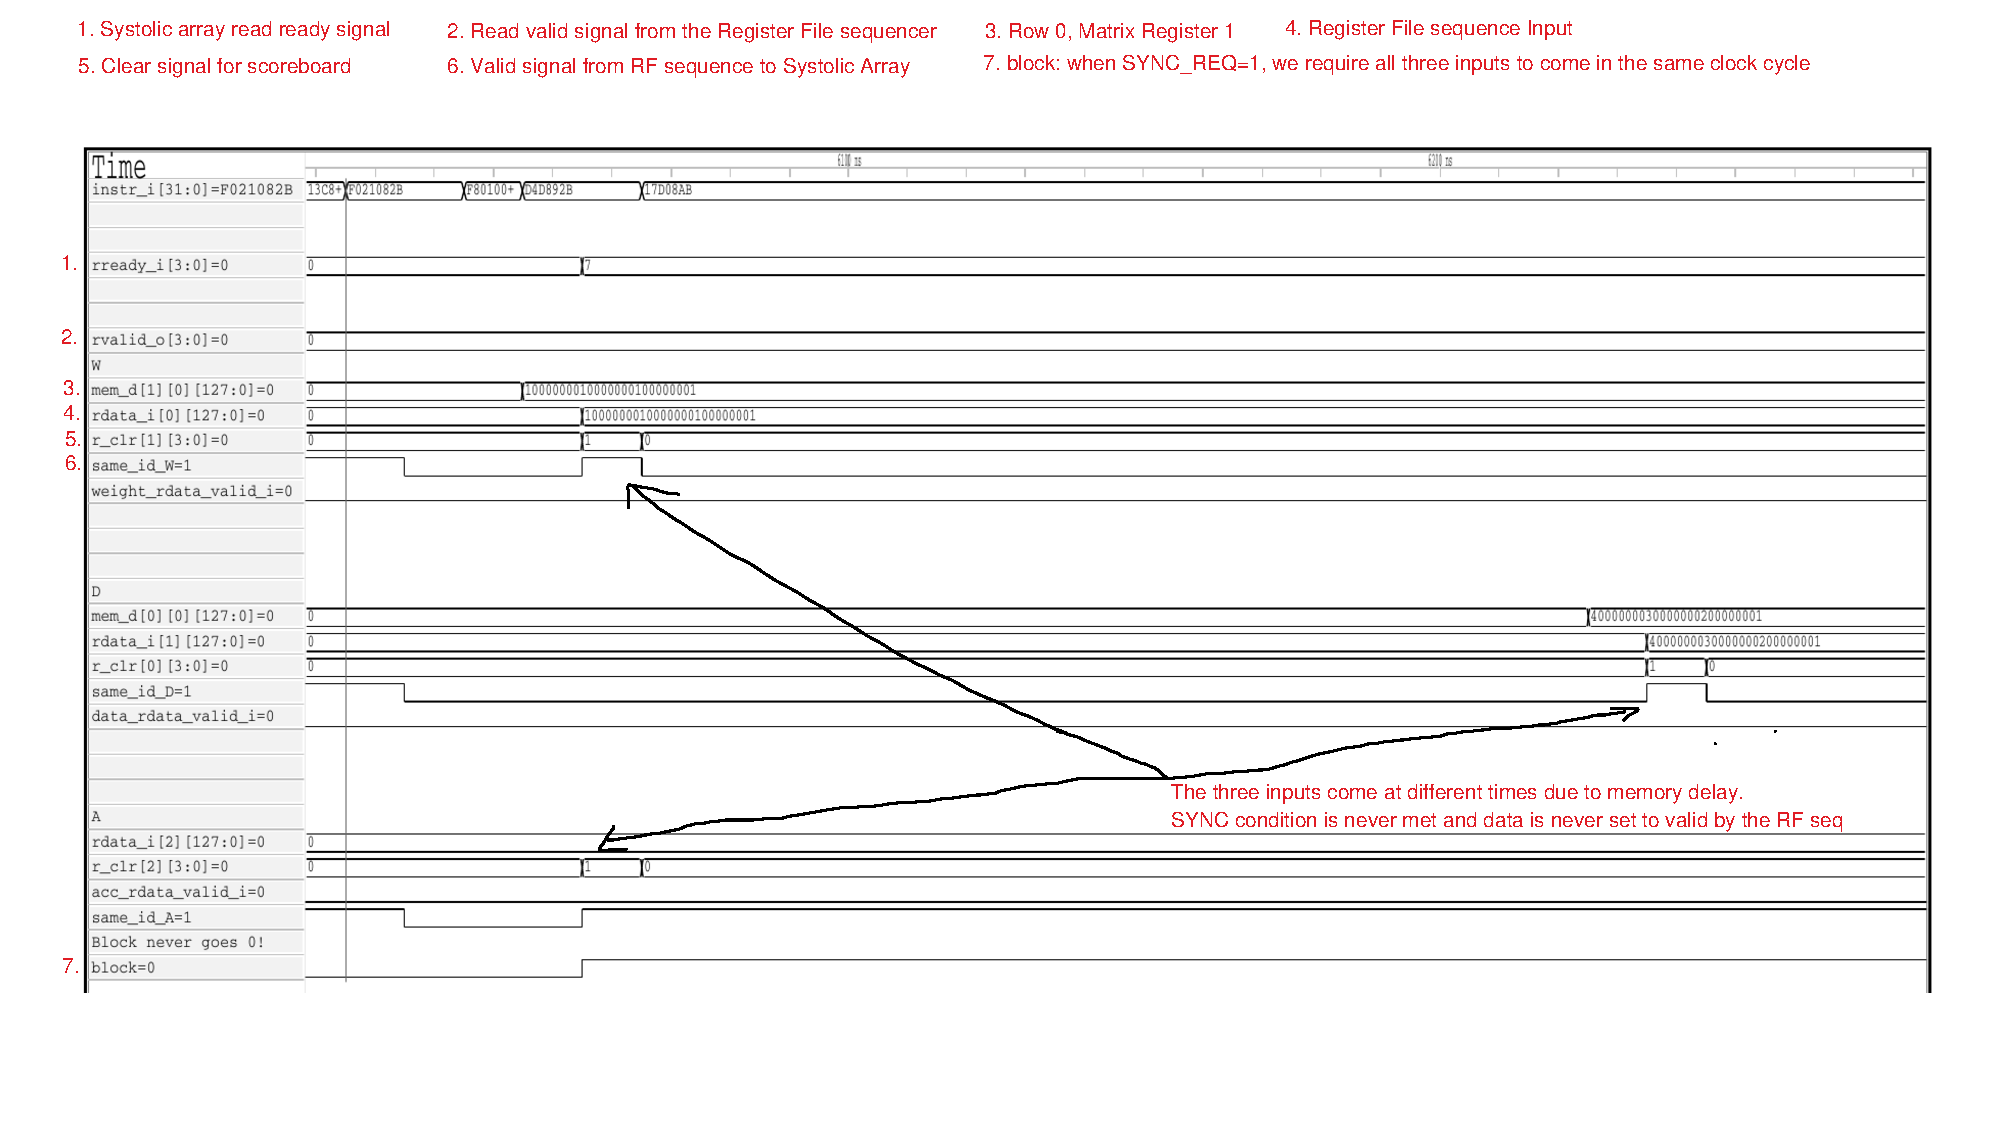
\includegraphics[width=\textwidth]{figures/original_with_sync_req_annotated.pdf}
  \caption{Waveform with \texttt{SYNC\_REQ=1}: the RF sequencer blocks forever
           while waiting for a synchronous data fetch}
  \label{fig:waveform_sync1}
\end{figure*}

The Register File Sequencer (RF sequencer) is an interface between the systolic array and
the register file. It validates accesses to the register file by the systolic array using a scoreboard
mechanism.

\begin{lstlisting}[
  language=Verilog,
  numbers=left,
  firstnumber=1,
  caption={RF sequencer blocking logic with \texttt{SYNC\_REQ=1}.},
  label=lst:sync_req,
  escapeinside={(*@}{@*)},
]
if(SYNC_REQ) begin: sa_sync_req
  logic block      ; (*@\label{lst:block_decl}@*)
  logic same_id_acc;
  logic same_id_A  ;
  logic same_id_D  ;
  logic same_id_W  ;
  same_id_A = rd_id_i[quadrilatero_pkg::SYSTOLIC_ARRAY_A] (*@\label{lst:sameA}@*)
            == scoreboard_q[raddr_i[quadrilatero_pkg::SYSTOLIC_ARRAY_A]]
                           [rrowaddr_i[quadrilatero_pkg::SYSTOLIC_ARRAY_A]].id;
  same_id_D = rd_id_i[quadrilatero_pkg::SYSTOLIC_ARRAY_D] (*@\label{lst:sameD}@*)
            == scoreboard_q[raddr_i[quadrilatero_pkg::SYSTOLIC_ARRAY_D]]
                           [rrowaddr_i[quadrilatero_pkg::SYSTOLIC_ARRAY_D]].id;
  same_id_W = rd_id_i[quadrilatero_pkg::SYSTOLIC_ARRAY_W] (*@\label{lst:sameW}@*)
            == scoreboard_q[raddr_i[quadrilatero_pkg::SYSTOLIC_ARRAY_W]]
                           [rrowaddr_i[quadrilatero_pkg::SYSTOLIC_ARRAY_W]].id;
  if( (*@\label{lst:blockif}@*)
      (rready_i[quadrilatero_pkg::SYSTOLIC_ARRAY_A] && !same_id_A) || (*@\label{lst:blockA}@*)
      (rready_i[quadrilatero_pkg::SYSTOLIC_ARRAY_D] && !same_id_D) || (*@\label{lst:blockD}@*)
      (rready_i[quadrilatero_pkg::SYSTOLIC_ARRAY_W] && !same_id_W)   (*@\label{lst:blockW}@*)
    ) begin
    block = 1'b1; (*@\label{lst:block1}@*)
  end else begin
    block = 1'b0; (*@\label{lst:block0}@*)
  end
\end{lstlisting}
By default, $\texttt{SYNC\_REQ} = 1$. From Lines~\ref{lst:blockif}--\ref{lst:block1} in
Listing~\ref{lst:sync_req}, the RF sequencer blocks until all three data lines are fetched
synchronously. Waveform~\ref{fig:waveform_sync1} shows that the \texttt{D} data line takes
longer to fetch (due to sequential memory access), so \texttt{block} is permanently set to $1$
and the pipeline stalls indefinitely.

\subsection{Disabling Synchronized Requests}
\begin{figure*}[t]
  \centering
  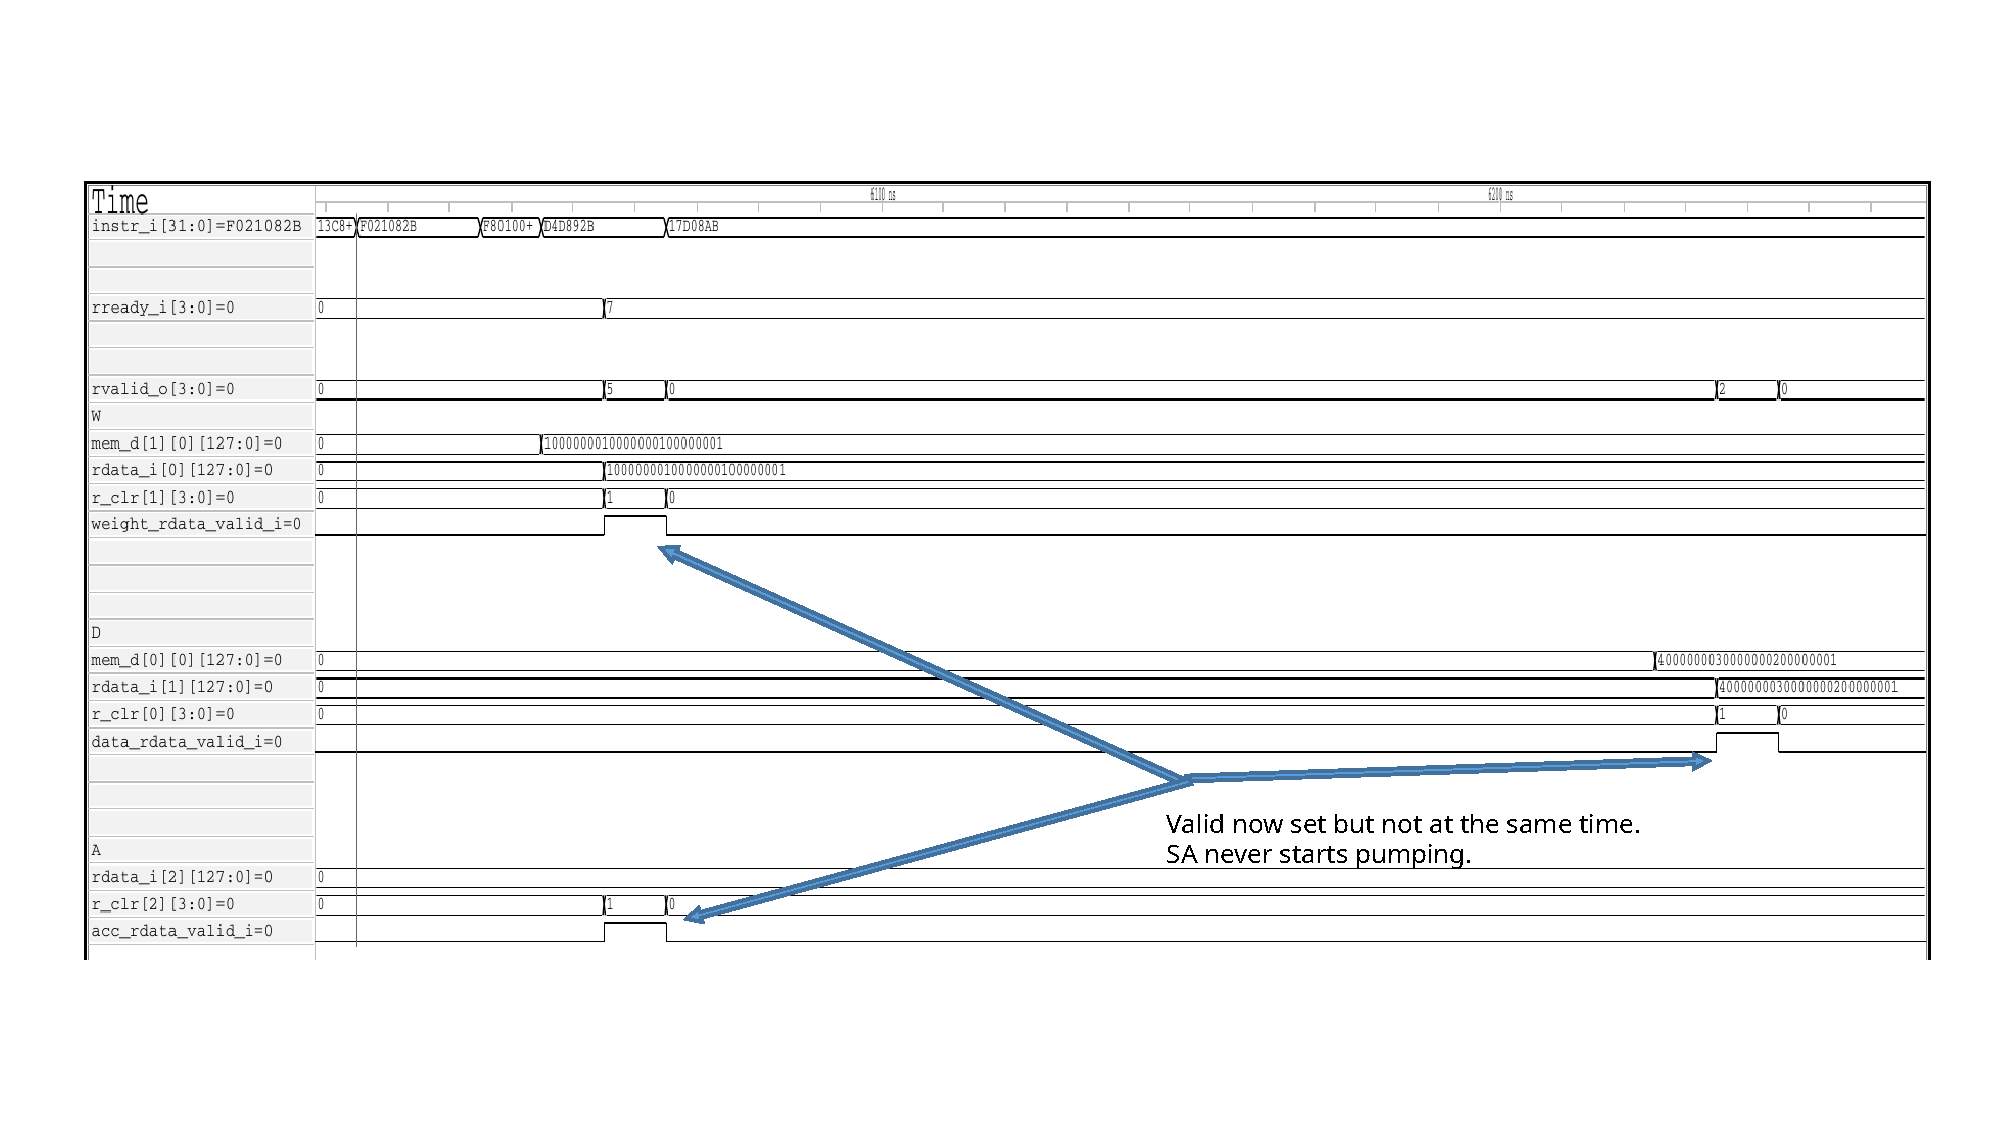
\includegraphics[width=\textwidth]{figures/original_wo_sync_req_annotated.pdf}
  \caption{Waveform with \texttt{SYNC\_REQ=0}: the systolic array always asserts \texttt{ready},
           causing data to be popped out of the scoreboard as soon as it is available.}
  \label{fig:waveform_sync0}
\end{figure*}
With \texttt{SYNC\_REQ=0}, waveform~\ref{fig:waveform_sync0} shows that the individual data
lines become valid at different times. Each line is only valid for one clock cycle before it
is popped from the scoreboard queue. This happens because the systolic array holds
\texttt{rready\_i} high permanently, so the handshake completes as soon as data arrives on
any given line, regardless of the other lines.

\begin{lstlisting}[
  language=Verilog,
  numbers=left,
  firstnumber=1,
  caption={RF output logic (\texttt{SYNC\_REQ=0}) in systolic array.},
  label=lst:rf_block,
  escapeinside={(*@}{@*)},
]
always_comb begin: rf_block
  // Weight Read Register Port
  weight_rdata_ready_o = ff_active_q &~ mask_req  ; (*@\label{lst:w_ready}@*)
  ...
  // Data Read Register Port
  data_rdata_ready_o   = ff_active_q  &~ mask_req ; (*@\label{lst:d_ready}@*)
  ...
  // Accumulator Read Register Port
  acc_rdata_ready_o    = ff_active_q &~ mask_req  ; (*@\label{lst:a_ready}@*)
  ...
end
\end{lstlisting}
From Listing~\ref{lst:rf_block} Line~\ref{lst:w_ready}, \texttt{weight\_rdata\_ready\_o} is set whenever the Feed First(FF) stage is active.
\begin{lstlisting}[
  language=Verilog,
  numbers=left,
  firstnumber=1,
  caption={Control logic of the systolic array. },
  label=lst:ctrl_block,
  escapeinside={(*@}{@*)},
]
always_comb begin: ctrl_block
  valid = weight_rdata_valid_i & data_rdata_valid_i & acc_rdata_valid_i; (*@\label{lst:valid}@*)
  clear = ~ff_active_q & ~fs_active_q & ~dr_active_q;
  ...
  ff_enable = ff_active_q &  valid                ; (*@\label{lst:ff_enable}@*)
  pump     = ff_enable | fs_enable | dr_enable                              ; (*@\label{lst:pump}@*)
  mask_req = (dr_counter_q==$clog2(MESH_WIDTH)'(MESH_WIDTH-1))
           & finished_q & ~finished_ack_i                                   ; (*@\label{lst:mask_req}@*)
end
\end{lstlisting}
However, the control logic requires all three data lines to be valid simultaneously
(Listing~\ref{lst:ctrl_block}, Line~\ref{lst:valid}). Since they never arrive at the same
cycle, \texttt{valid} is never asserted and the systolic array never begins pumping
(Listing~\ref{lst:ctrl_block}, Line~\ref{lst:pump}).

\subsection{Fixing Ready-Valid Handshake}
\begin{figure*}[t]
  \centering
  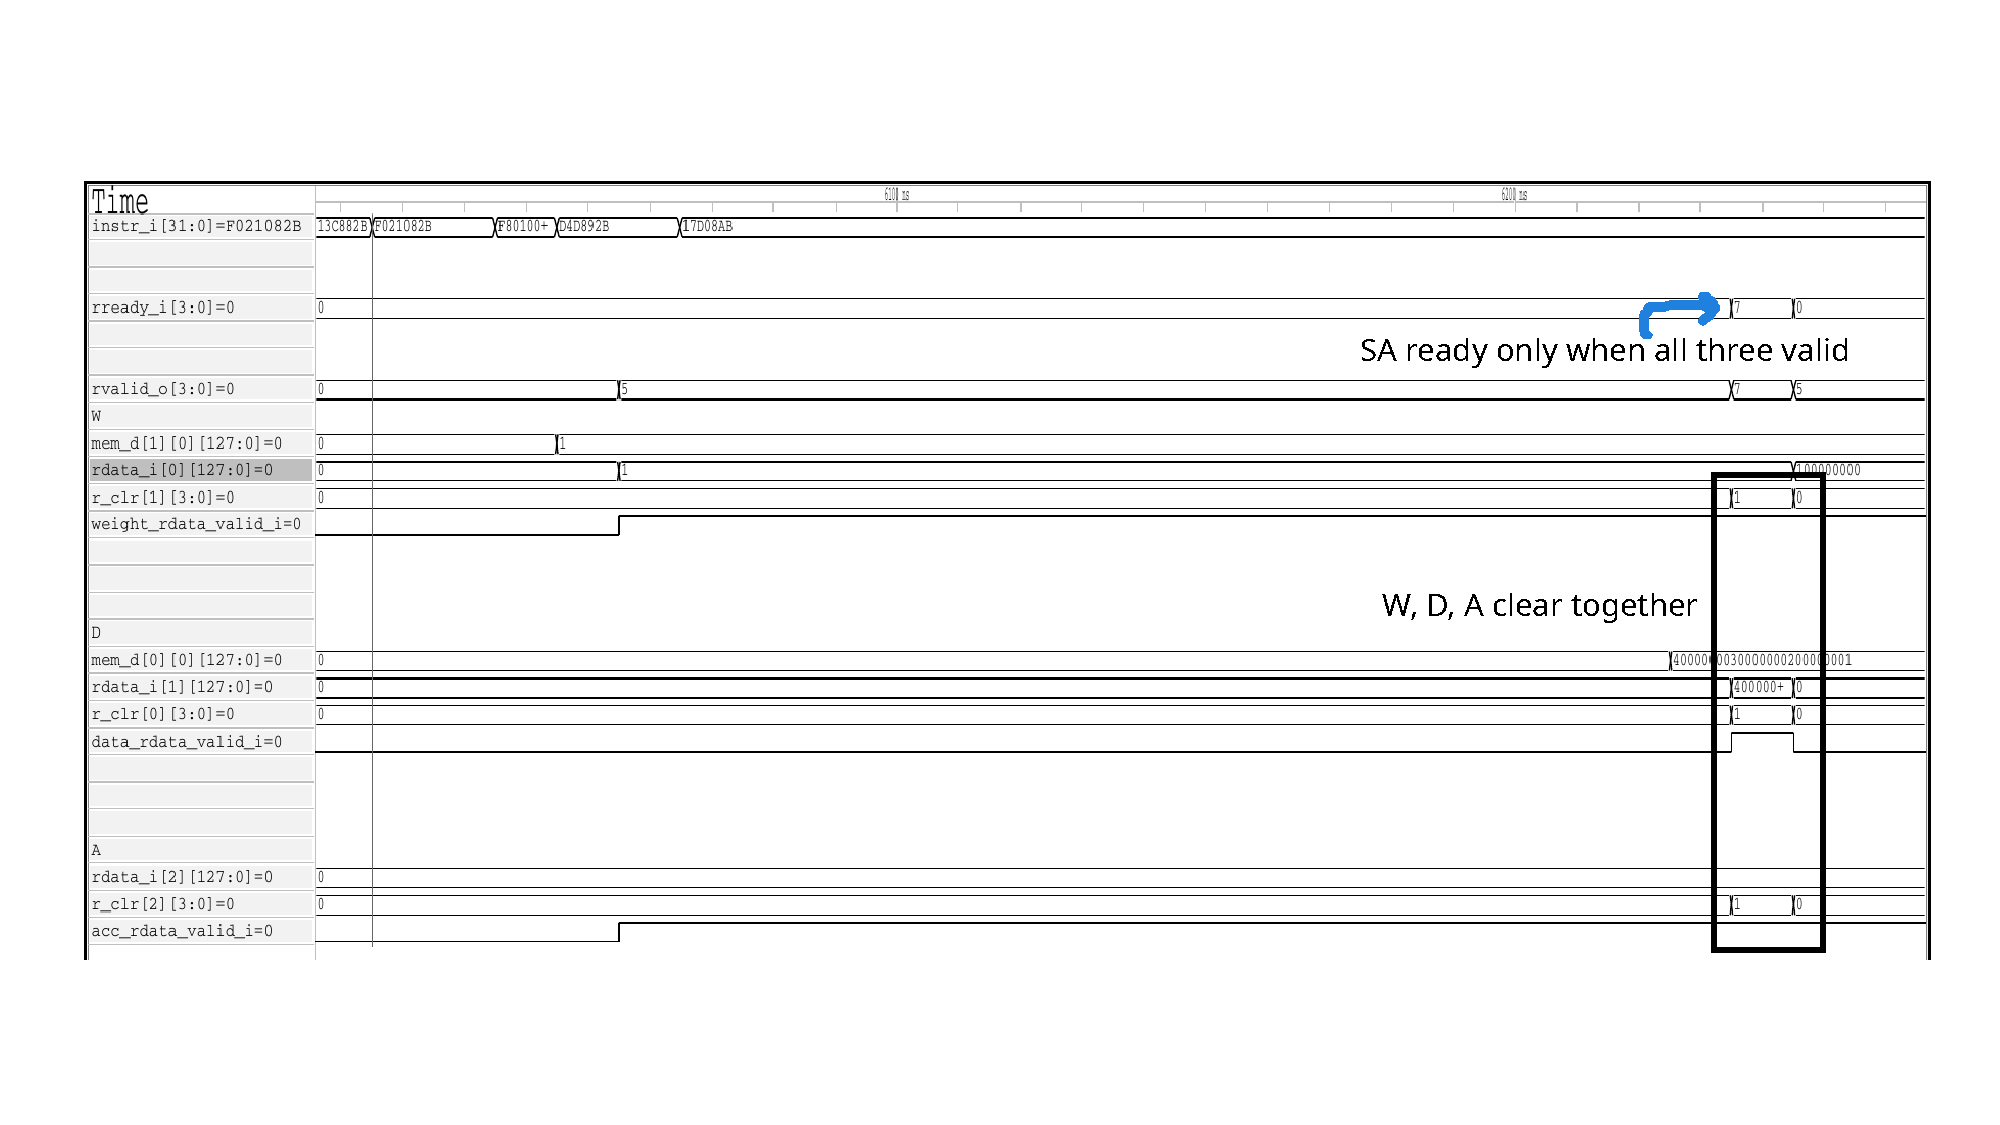
\includegraphics[width=\textwidth]{figures/final_annotated.pdf}
  \caption{Waveform of a working simulation. \texttt{Valid} set independently by RF sequencer. Systolic array sets \texttt{Ready} when \texttt{Valid} is set.}
  \label{fig:final}
\end{figure*}

The fix is to change the control logic so that \texttt{rready\_i} is only asserted once all
three data lines are valid, while each line's valid is raised independently as soon as that
line's data is available. This is the standard ready-valid handshake: the producer drives
valid when its data is ready; the consumer drives ready when it can accept all inputs.
\begin{lstlisting}[
  language=Verilog,
  numbers=left,
  firstnumber=1,
  caption={Fixed RF output logic (\texttt{SYNC\_REQ=0}) in systolic array.},
  label=lst:rf_block_fixed,
  escapeinside={(*@}{@*)},
]
always_comb begin: rf_block
  // Weight Read Register Port
  weight_rdata_ready_o = ff_enable &~ mask_req  ; (*@\label{lst:w_ready}@*)
  ...
  // Data Read Register Port
  data_rdata_ready_o   = ff_enable  &~ mask_req ; (*@\label{lst:d_ready}@*)
  ...
  // Accumulator Read Register Port
  acc_rdata_ready_o    = ff_enable &~ mask_req  ; (*@\label{lst:a_ready}@*)
  ...
end
\end{lstlisting}


% =========================================================
\section{Results}
\label{sec:results}

\begin{figure}[htbp]
  \centering
  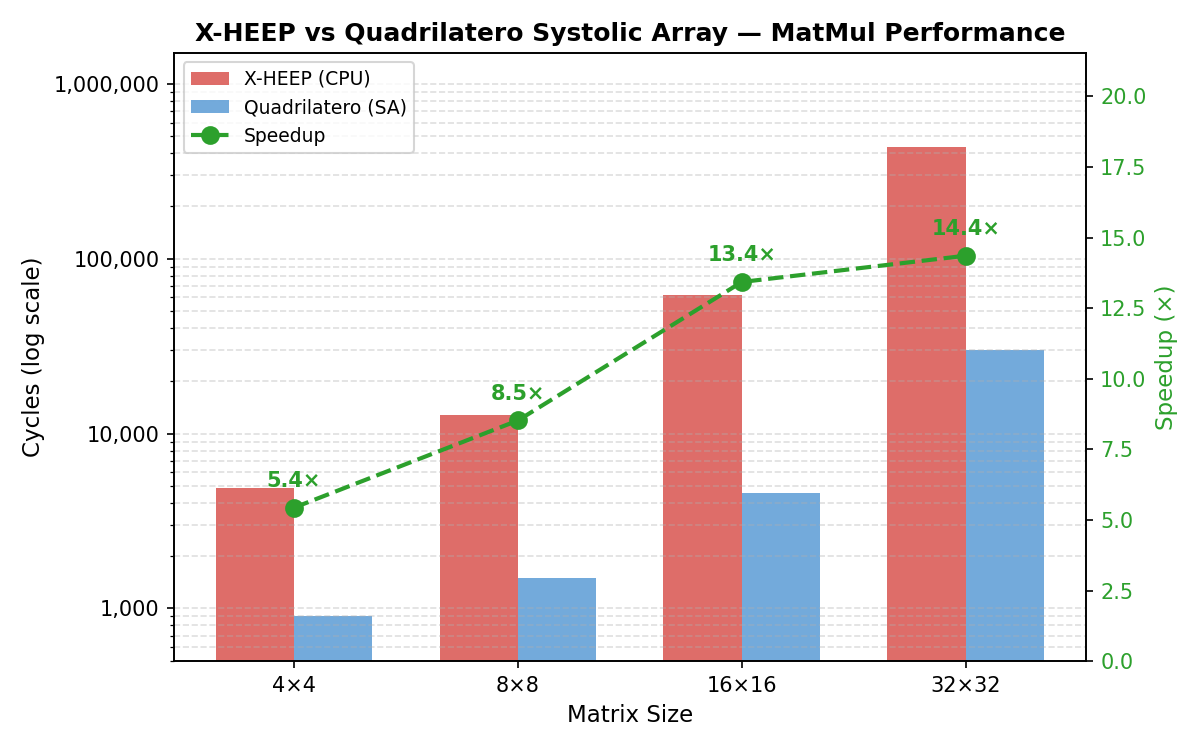
\includegraphics[width=\columnwidth]{../results.png}
  \caption{Cycle counts for scalar (\texttt{example\_matmul}) vs.\
           accelerated (\texttt{example\_matmul\_quadrilatero}) matrix
           multiply across input sizes.}
  \label{fig:results}
\end{figure}

The measured speedup over the scalar baseline is lower than the
${\sim}5\times$ reported in the Quadrilatero paper~\cite{quadrilatero2021}.
The likely cause is that the Weight-Load-Select (WLS) optimisation, which
overlaps weight loading with computation, was disabled during debugging to
rule out a source of correctness issues. Re-enabling WLS should close the gap.

\begin{table}[htbp]
  \centering
  \caption{Verified simulation results. Cycle counts are approximate.
           Speedup is relative to the scalar baseline.}
  \label{tab:results}
  \begin{tabular}{@{}lccc@{}}
    \toprule
    \textbf{Matrix size} & \textbf{Scalar (cycles)} &
    \textbf{Accel.\ (cycles)} & \textbf{Speedup} \\
    \midrule
    4$\times$4   & 4902 & 902 & 5.43 \\
    8$\times$8   & 12802 & 1502 & 8.52 \\
    16$\times$16 & 61802 & 4602 & 13.43 \\
    32$\times$32 & 433702 & 30202 & 14.36 \\
    \bottomrule
  \end{tabular}
\end{table}

% =========================================================
\section{Conclusion}
\label{sec:conclusion}

This report surveyed four candidate platforms for running a Hardware
Processing Engine on an FPGA using an open-source toolchain. Google Coral
was rejected immediately for lacking an FPGA flow. PULPissimo was rejected
because its SDK is end-of-life and its simulation flow mandates QuestaSim.
Six PULP-derived alternatives were surveyed; all lacked either FPGA support
or a compatible compiler backend.

X-HEEP extended with Quadrilatero satisfies all three selection criteria: it
has first-class FPGA support, a fully open-source Docker-based toolchain, and
a well-specified CV-X-IF accelerator interface that allows the co-processor
to be integrated without modifying MCU RTL. 

The main takeaway from this survey is that software ecosystem maturity matters
as much as hardware quality. PULPissimo's hardware is well-designed; the problem
is that the software around it has gone stale. X-HEEP's Docker image, Verilator
flow, and Makefile build system made it possible to go from a blank machine to a
verified simulation.

Open problems include FPGA hardware validation against the simulation and
integration of the Deeploy compiler framework to enable deployment of full neural
network layers from high-level representations.

% =========================================================
\bibliographystyle{IEEEtran}
\nocite{*}
\bibliography{references}

\end{document}
